\documentclass{standalone}
\usepackage{tikz}

\begin{document}

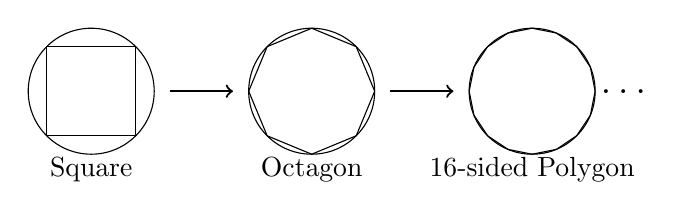
\begin{tikzpicture}[scale=0.4]
    % Draw the first part: a circle with a square inscribed
    \draw (0, 0) circle (2); % Draw the outer circle
    \draw (-1.414, 1.414) -- (1.414, 1.414) -- (1.414, -1.414) -- (-1.414, -1.414) -- cycle; % Draw the square
    \node at (0, -2.5) {Square};
    
    % Draw an arrow to the right
    \draw[->, thick] (2.5, 0) -- (4.5, 0);
    
    % Draw the second part: a circle with an octagon inscribed
    \begin{scope}[shift={(7, 0)}]
        \draw (0, 0) circle (2); % Draw the outer circle
        \foreach \i in {0, 45, 90, 135, 180, 225, 270, 315} {
            \pgfmathsetmacro\xA{2 * cos(\i)}
            \pgfmathsetmacro\yA{2 * sin(\i)}
            \pgfmathsetmacro\xB{2 * cos(\i+45)}
            \pgfmathsetmacro\yB{2 * sin(\i+45)}
            \draw (\xA, \yA) -- (\xB, \yB); % Draw the octagon sides
        }
        \node at (0, -2.5) {Octagon};
    \end{scope}
    
    % Draw another arrow to the right
    \draw[->, thick] (9.5, 0) -- (11.5, 0);
    
    % Draw the third part: a circle with a 16-sided polygon inscribed
    \begin{scope}[shift={(14, 0)}]
        \draw (0, 0) circle (2); % Draw the outer circle
        \foreach \i in {0, 22.5, 45, 67.5, 90, 112.5, 135, 157.5, 180, 202.5, 225, 247.5, 270, 292.5, 315, 337.5} {
            \pgfmathsetmacro\xA{2 * cos(\i)}
            \pgfmathsetmacro\yA{2 * sin(\i)}
            \pgfmathsetmacro\xB{2 * cos(\i+22.5)}
            \pgfmathsetmacro\yB{2 * sin(\i+22.5)}
            \draw (\xA, \yA) -- (\xB, \yB); % Draw the 16-sided polygon sides
        }
        \node at (0, -2.5) {16-sided Polygon};
    \end{scope}

    % Draw ellipses to indicate continuation
    \node at (17, 0) {\Large \dots};
    
\end{tikzpicture}

\end{document}
